\documentclass[ThesisDJ.tex]{subfiles}

\begin{document}
	Das Projekt zur Evaluation verschiedener Softwarelösungen zur Verbesserung der Kommunikation innerhalb von Teams bzw. Verfahren im Bereich J3 wird zwar im Bereich J3 durchgeführt, hängt aber von keinem der existierenden Projekte, Verfahren oder auch Personen insofern ab, als dass sie direkt als Projektmitarbeiter in das Projekt involviert sind. Somit besteht für die Wahl der Arbeitsweise freie Hand und es ist dem Projektteam überlassen, eine passende Arbeitsweise auszuwählen und in der Folge anzuwenden.\\
	Da der Projektauftrag klar definiert und die zur Verfügung stehende Arbeitszeit durch die Laufzeit stark begrenzt ist, wird weitestgehend traditionell gearbeitet, wobei allerdings Änderungen bzw. weitere notwendige Arbeit nach Bedarf auch nachträglich in die Planung eingebracht werden kann, ohne alle Planungsschritte erneut zu durchlaufen. Einzelne Arbeitsschritte können aber auch agil bearbeitet werden, wenn dies für die Durchführung des Arbeitsschrittes voraussichtlich förderlich ist.
	
	\subsection{Projektbewertung und -beschreibung}
	Die Zusammenarbeit innerhalb und zwischen Teams im Bereich J3, insbesondere zwischen Mitarbeitern im Büro und Mitarbeitern, die per mobilem Arbeiten von Zuhause arbeiten findet aktuell über eine Vielzahl verschiedener Plattformen statt. Zur direkten Kommunikation werden entweder Mails über Microsoft Outlook oder Nachrichten und Sprachanrufe über Skype eingesetzt, ganze Teams können dabei über die dem Team zugeordneten Mail-Postfächer direkt gesammelt angesprochen werden. Ebenso findet Skype Anwendung bei der Durchführung von Videokonferenzen. Tickets und Changes werden mittels Remedy erstellt und bearbeitet. In Projekt-Teams wird zur Planung und Durchführung Azure DevOps verwendet. \\
	Diese Vielzahl an eingesetzten Programmen bringt Herausforderungen in der Koordination mit sich im Hinblick auf Aufgabenverteilung, Absprache und Abstimmung von Resultaten verschiedener Arbeitspakete, die sich nicht unter Einsatz der bereits verwendeten Programme lösen lässt.
	Gesucht wird also ein Programm, das eine Schnittstelle zwischen den bereits eingesetzten Tools darstellt und gleichzeitig eine gut strukturierbare Möglichkeit zur Kommunikation innerhalb eines Teams sowie teamübergreifend bietet, so dass sich die Zusammenführung der eingesetzten Programme effizienzsteigernd auswirkt.
	
	\subsection{Ziele}
	Das Projekt verfolgt zwei Ziele, wobei das zweite Ziel vom ersten Ziel abhängig ist.
	Das erste Ziel ist eine Empfehlung für eine Softwarelösung, mit der die Zusammenarbeit innerhalb eines Projekt- oder Verfahrens-Teams verbessert werden soll, insbesondere bei einer Aufteilung des Teams in Mitarbeiter, die vor Ort im Büro arbeiten und in Mitarbeiter, die per mobilem Arbeiten von zuhause aus arbeiten und somit nicht persönlich im Büro erreichbar sind, abzugeben.\\
	Dafür soll eine Evaluation verschiedener Softwarelösung angestellt und anschließend ausgewertet werden, sodass die Empfehlung transparent nachvollzogen werden kann.\\
	Das zweite Ziel ist die Erstellung und Dokumentation eines Proof of Concept, bei dem die das erste Ziel darstellende Softwarelösung eingesetzt und so konfiguriert wird, dass sie für den Bereich J3 eingesetzt werden kann. Ergebnis davon soll die Dokumentation in Form eines Wikis sowie eine Konfigurationsanleitung sein, die eine Nachbildung des Proof of Concept ermöglicht.
	
	
	\subsection{Projektauftrag}
	
	Der Projektauftrag gliedert sich in mehrere Punkte, die im Folgenden beschrieben sind:\bigskip\\
	\textbf{Zielsetzung:}\medskip\\
	Wie bereits im Kapitel zu den Zielen ausführlich beschrieben, bestehen zwei Ziele für das Projekt. Nach einer Evaluation verschiedener Softwarelösungen, die eine Empfehlung für eine der evaluierten Lösungen zum Ziel hat, soll als zweites Ziel die Software, für die eine Empfehlung ausgesprochen wurde ein Proof of Concept aufgesetzt werden, zu dem eine Konfigurationsanleitung für den praktischen Einsatz erstellt wird, die dann vom Bereich J3 verwendet werden kann.\bigskip\\
	\textbf{Vorgehensplan:}\medskip\\
	Als Vorgehensplan wurden initial Meilensteine aufgestellt und mit Terminen versehen, zu denen sie abgeschlossen sein sollten. Diese Meilensteine sowie weitere Details zur Zeitplanung werden im entsprechenden Kapitel näher erläutert.\bigskip\\
	\textbf{Abhängigkeiten und Einflussgrößen:}	\medskip\\
	Wie in der Stakeholdermatrix (Link zu Bild/Kapitel) zu sehen ist, existieren verschiedene Stakeholder, die allerdings alle innerhalb der HZD zu verorten sind. Da es sich beim beschriebenen Projekt um ein Projekt innerhalb des Bereichs J3 handelt, dessen Resultat primär auch nur in diesem Bereich eingesetzt werden soll, werden alle Stakeholder, die außerhalb des Bereichs J3 angesiedelt sind, als externe Stakeholder betrachtet. Dies ermöglicht eine genauere Differenzierung der verschiedenen Stakeholder innerhalb der HZD.\bigskip\\
	\textbf{Personalressourcen und Projektorganisation:}\medskip\\
	Für das Projekt stehen 3 Duale Studenten der HZD im Bereich J3 im Projektzeitraum jeweils einen Tag in der Woche zur Verfügung, es kann also mit 3 Personentagen pro Woche für den gesamten Projektzeitraum gerechnet werden, in der Summe sind das 45 Personentage.
	Aufgrund der sehr kleinen Teamgröße gibt es keinen festen Projektleiter, das Vorgehen und die Aufgabenverteilung werden in gemeinsamen Besprechungen festgelegt und miteinander abgestimmt.\bigskip\\
	\textbf{Schätzung der Projektkosten:}\medskip\\
	Die Projektkosten selbst beschränken sich weitestgehend auf die Personalkosten der Projektmitarbeiter.
	Es muss für das Projekt keine zusätzliche Hardware angeschafft werden, an Kosten für Software fällt gegebenenfalls die Lizenzgebühr für die im Proof of Concept zu betrachtende Software an.\bigskip\\
	\textbf{Rahmenbedingungen und Risiko:}\medskip\\
	Wie bei den Personalressourcen bereits beschrieben ist ein wichtiger Faktor im Projekt die geringe wöchentliche Arbeitszeit am Projekt aller Teammitglieder von einem Arbeitstag pro Woche.\\	
	In der HZD wird aktuell ein Wechsel von Skype zu Webex als Kommunikationsplattform erwogen. Wenn dieser Wechsel erfolgt, könnte die Nutzung einer zusätzlichen Softwarelösung obsolet werden, da mit Webex ein Teil der von der Softwarelösung geforderten Funktionen bereits abdeckt werden und sich der Aufwand, für die verbleibenden Funktionen eine zusätzliche Software zu verwenden gegebenenfalls nicht lohnt. Somit ist ein Wechsel zu Webex ein Projektrisiko, da dadurch das Projektergebnis nutzlos werden könnte. 
	\subsection{Stakeholder}
  \begin{figure}[h!]
    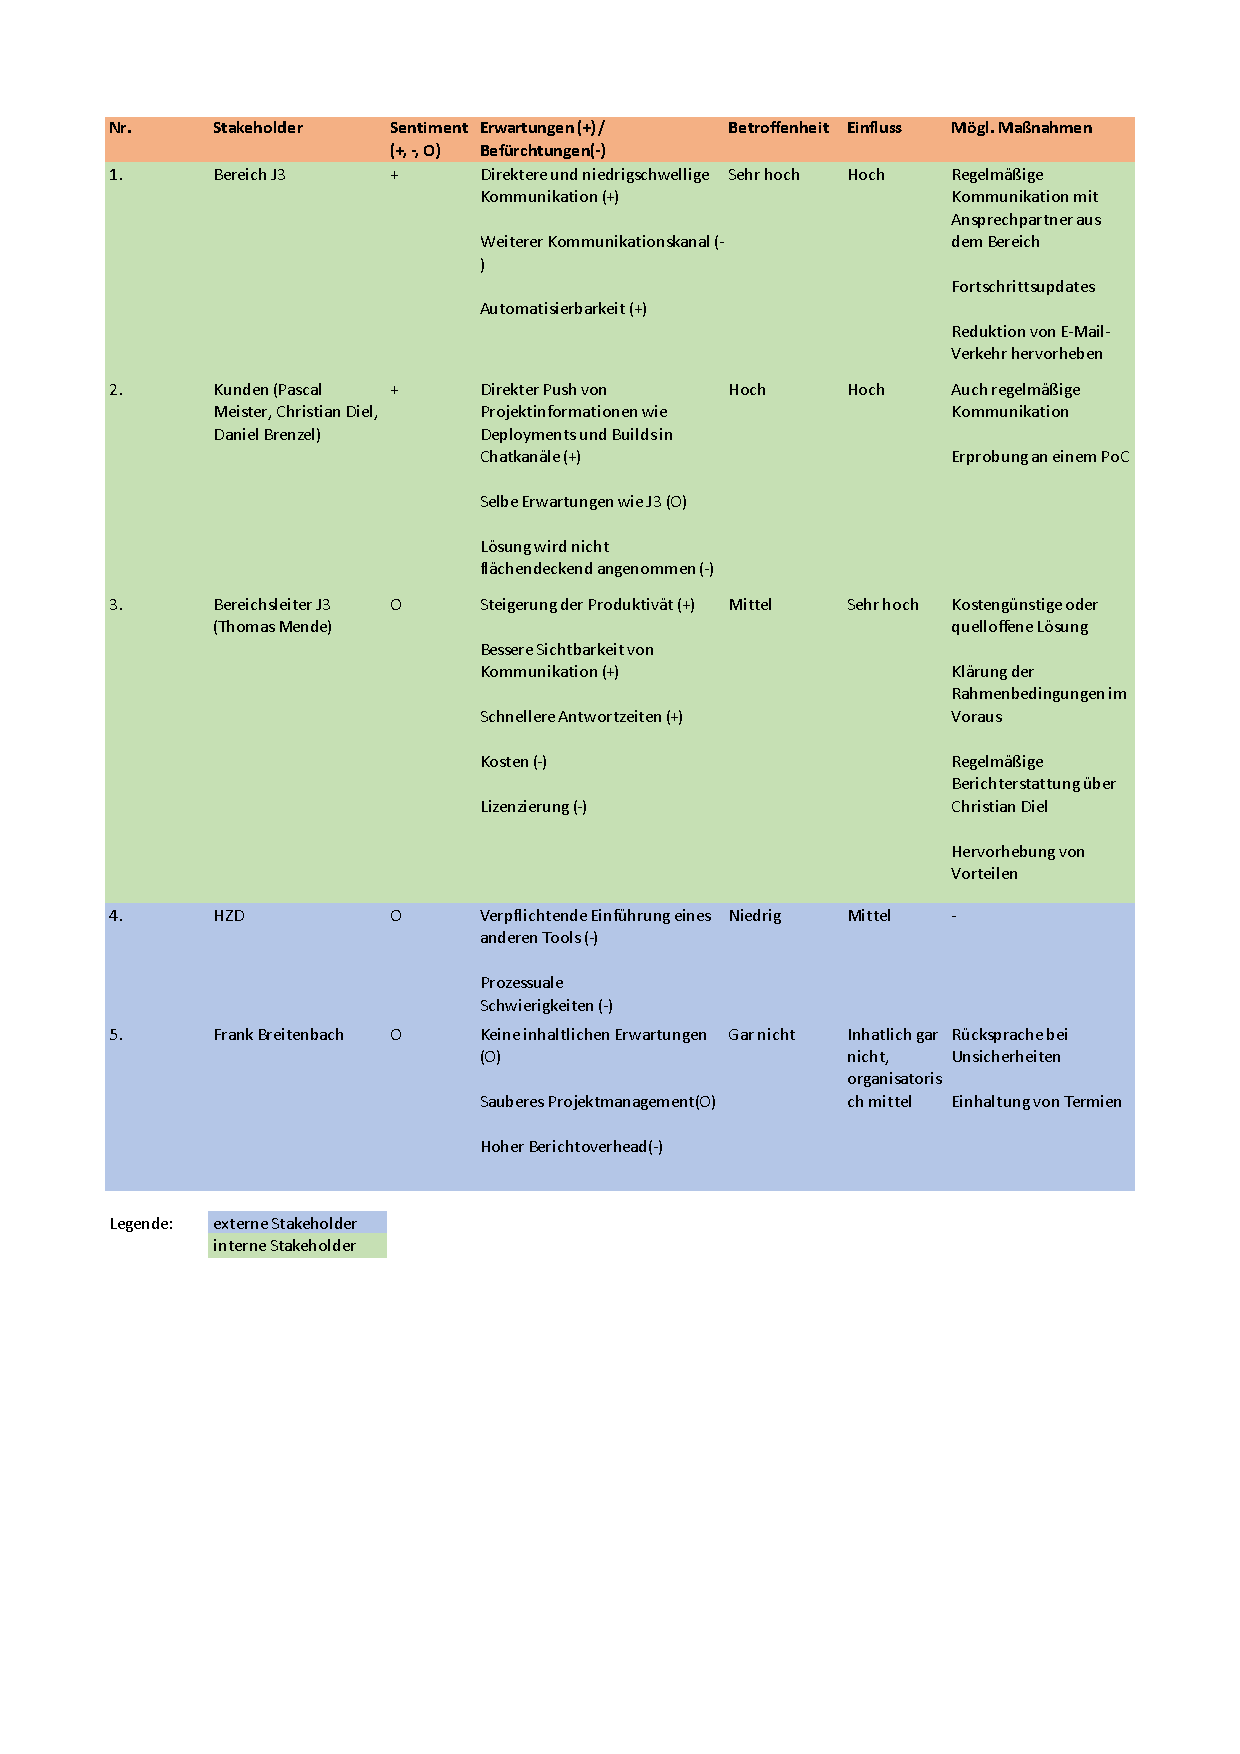
\includegraphics[width=\textwidth]{Stakeholdermatrix.pdf}
    \centering
    \caption{Stakeholdermatrix des Projekts}
    \label{fig:stakeholders}
  \end{figure}

  Um einen Überblick über die Betroffenen des Projekts zu gewinnen, wurde eine Stakeholdermatrix angefertigt. Sie fasst die Beteiligten zusammen, indem sie ihre Einstellungen zu dem Projekt sowie mögliche Erwartungen und Befürchtungen auflistet. Außerdem wird der Einfluss der jeweiligen Stakeholder auf das Projekt abgeschätzt und mögliche Maßnahmen zur Beeinflussung aufgeführt. Die Matrix ist nach internen (grün) und externen (blau) Stakeholdern aufgeteilt. 

	
	\subsection{Dokumentationsform}
	
	Die Lieferobjekte des Projekts bestehen, wie im Projekt-Canvas ebenfalls zu sehen sein wird, aus einer Entscheidung für ein einzusetzendes Programm, das den Zweck der verbesserten Kommunikation erfüllt, zusammen mit einer Dokumentation des Evaluationsprozesses sowie einem Proof of Concept zur Konfiguration der ausgewählten Software.\\
	Dementsprechend wird die Dokumentation ebenfalls zweigeteilt sein. Der erste Teil wird abgedeckt durch die Dokumentation des Evaluationsprozesses, die Teil des Lieferobjektes ist, im zweiten Teil wird der Proof of Concept dokumentiert in Form einer Wiki, die die Nutzung und insbesondere die Konfiguration des gewählten Programms beschreibt. 
	
	\subsection{Projekt-Canvas}
	<insert Projekt-Canvas>
\end{document}
